% IEEE Conference Template for ML/AI Papers
% Document class specification - conference format for IEEE
\documentclass[conference]{IEEEtran}

% Override command lockouts (typically needed for IEEE papers)
\IEEEoverridecommandlockouts
% The preceding line is only needed to identify funding in the first footnote. If that is unneeded, please comment it out.

%%%%%%%%%%%%%%%%%%%%%%%%%%%%%%%%%%%%%%%%%
% PACKAGES
%%%%%%%%%%%%%%%%%%%%%%%%%%%%%%%%%%%%%%%%%
% Citation management
\usepackage{cite}                    % For bibliography citations
\usepackage[T1]{fontenc}            % Better font encoding for BibTeX names

% Text and list formatting
\usepackage{enumitem}                % Enhanced list environments
\usepackage{amsmath,amssymb,amsfonts} % Mathematical symbols and fonts

% Algorithms
\usepackage{algorithm}               % For algorithm environments
\usepackage{algorithmic}             % For algorithm formatting

% Graphics and visual elements
\usepackage{graphicx}                % For including images
\usepackage{textcomp}                % Text companion fonts
\usepackage{xcolor}                  % For colored text
\usepackage{forest}                  % For drawing tree diagrams

% TikZ and related packages for diagrams
\usepackage{tikz}                    % Core package for creating graphics
\usepackage{adjustbox}               % For scaling figures
\usepackage{url}                     % For formatting URLs

% Figure and table enhancements
\usepackage{pgfplots}                % For creating plots
\usepackage{booktabs}                % For professional-looking tables
\usepackage{colortbl}                % For colored table cells
\pgfplotsset{compat=1.18}

% TikZ libraries for specific diagram types
\usetikzlibrary{shapes.geometric,arrows,positioning,fit,backgrounds,calc,decorations.pathreplacing,decorations.markings,patterns,circuits.logic.US,matrix,chains}

% Table enhancements
\usepackage{threeparttable}          % For table notes
\usepackage{cuted}                   % For multi-column environments

% Custom command for line breaks in author block
\makeatletter
\newcommand{\linebreakand}{%
  \end{@IEEEauthorhalign}
  \hfill\mbox{}\par
  \mbox{}\hfill\begin{@IEEEauthorhalign}
}
\makeatother

% Define custom colors for visualizations
% These are common colors used in AI/ML papers
\definecolor{qubitblue}{RGB}{70,130,180}      % Blue for primary elements
\definecolor{controlred}{RGB}{220,20,60}      % Red for control elements
\definecolor{aigreen}{RGB}{50,150,50}         % Green for AI components
\definecolor{quantumpurple}{RGB}{128,0,128}   % Purple for quantum elements
\definecolor{errororange}{RGB}{255,140,0}     % Orange for error highlighting

%%%%%%%%%%%%%%%%%%%%%%%%%%%%%%%%%%%%%%%%%
% DOCUMENT BEGINS
%%%%%%%%%%%%%%%%%%%%%%%%%%%%%%%%%%%%%%%%%
\begin{document}

%%%%%%%%%%%%%%%%%%%%%%%%%%%%%%%%%%%%%%%%%
% TITLE SECTION
%%%%%%%%%%%%%%%%%%%%%%%%%%%%%%%%%%%%%%%%%
\title{Parameter-Efficient Fine-Tuning for Large Language Models: A Survey (2022--2026)}

\author{
    \IEEEauthorblockN{
        Author Name
    }
    \IEEEauthorblockA{
        Affiliation
        \\ Email: author@example.com
    }
}

\maketitle

%%%%%%%%%%%%%%%%%%%%%%%%%%%%%%%%%%%%%%%%%
% KEYWORDS
%%%%%%%%%%%%%%%%%%%%%%%%%%%%%%%%%%%%%%%%%
\begin{IEEEkeywords}
parameter-efficient fine-tuning, PEFT, large language models, adapters, LoRA, quantized fine-tuning
\end{IEEEkeywords}

%%%%%%%%%%%%%%%%%%%%%%%%%%%%%%%%%%%%%%%%%
% ABSTRACT
%%%%%%%%%%%%%%%%%%%%%%%%%%%%%%%%%%%%%%%%%
\begin{abstract}
Parameter-efficient fine-tuning (PEFT) has become a default way to adapt foundation models when full fine-tuning is prohibitively expensive in memory, compute, or storage. Between 2022 and early 2026, PEFT evolved from early adapters and prompt-based tuning into a broad algorithmic design space that includes low-rank updates (the LoRA family), module composition and merging, and quantization-aware training pipelines such as QLoRA. This survey synthesizes the period with an algorithm-first perspective while covering language, vision, and multimodal/diffusion models. We introduce a unified ``delta'' view that cleanly separates frozen base parameters from trainable adaptation parameters, and we organize PEFT methods by how they parameterize and compose these deltas (additive modules, low-rank reparameterizations, prompt/prefix parameters, and selective tuning). We then distill recurring design choices---where to adapt, how to allocate parameter budgets, how to initialize and optimize, and whether updates are mergeable for deployment---and connect them to practical system constraints such as optimizer-state memory and serving-time overhead. Finally, we provide an evaluation checklist that jointly reports quality, cost, and reproducibility, and we discuss open challenges around multi-adapter composition, robustness under repeated adaptation, and safe/provenanced adapter sharing.
\end{abstract}

%%%%%%%%%%%%%%%%%%%%%%%%%%%%%%%%%%%%%%%%%
% INTRODUCTION
%%%%%%%%%%%%%%%%%%%%%%%%%%%%%%%%%%%%%%%%%
\section{Introduction}
Foundation models are increasingly adapted to new tasks, domains, and users via post-training. However, full fine-tuning scales training-time memory (e.g., optimizer states) and requires storing a full model copy per specialization, which is often infeasible for large language models (LLMs) and large vision/multimodal backbones \cite{han2024parameter,wang2024parameter,prottasha2025peft}. Parameter-efficient fine-tuning (PEFT) addresses this gap by keeping most pretrained parameters frozen and learning a comparatively small set of adaptation parameters, aiming to retain most of the benefits of fine-tuning while reducing training cost and storage overhead \cite{zhang2025parameter,han2024parameter}.

PEFT is not a single technique but a family of parameterizations for ``delta'' updates. Seminal foundations include adapter modules \cite{houlsby2019parameter,pfeiffer2020adapterhub}, prompt/prefix-based tuning that learns continuous task-specific inputs \cite{li2021prefix,lester2021the,liu2021p}, and selective tuning that updates only small subsets of parameters \cite{benzaken2021bitfit,liu2022few}. Low-rank reparameterizations such as LoRA popularized a simple and mergeable way to constrain updates in large transformer layers \cite{hu2021lora}, which subsequently inspired a fast-growing ecosystem of variants and analyses \cite{zhang2023adalora,liu2024dora,wang2024lora,hu2024computational}.

The 2022--2026 period also saw PEFT expand from ``NLP-only'' methods to a cross-modality toolkit. Vision and vision-language models are frequently adapted with prompt-like parameters and lightweight modules (e.g., visual prompt tuning and CLIP adapters) \cite{jia2022visual,zhang2021tip,radford2021learning}, and PEFT has become a standard adaptation primitive for diffusion models and diffusion transformers \cite{rombach2021high,ho2020denoising,huang2024in}. At the same time, quantization-aware pipelines such as QLoRA made it practical to fine-tune very large models on commodity hardware, which shifted the systems frontier and the set of ``reasonable defaults'' for practitioners \cite{dettmers2023qlora,han2024parameter}.

This survey focuses on research from 2022 through March~17,~2026, while including seminal pre-2022 work when needed for context \cite{han2024parameter,wang2024parameter}. Our emphasis is algorithmic: we propose a taxonomy organized by update parameterization and composition, summarize the design space (placement, budget allocation, initialization/optimization, and mergeability), and connect these choices to systems constraints and deployment patterns \cite{chen2023parameter,si2024see}. We also cover evaluation practices across language, vision, and multimodal settings and discuss emerging risks around safety, privacy, and provenance in low-cost adaptation \cite{taraghi2025efficiency,wang2025stolenlora}.

\begin{table}[t]
    \centering
    \caption{Representative PEFT milestones (selected; not exhaustive).}
    \label{tab:peft-timeline}
    \scriptsize
    \setlength{\tabcolsep}{3pt}
    \begin{tabular}{p{0.85cm}p{6.35cm}}
        \toprule
        \textbf{Year} & \textbf{Representative methods/ideas} \\
        \midrule
        2019 & Adapters for transfer learning \cite{houlsby2019parameter}. \\
        2020 & AdapterHub and AdapterFusion \cite{pfeiffer2020adapterhub,pfeiffer2020adapterfusion}. \\
        2021 & Prefix/prompt tuning; P-tuning v2; LoRA; BitFit \cite{li2021prefix,lester2021the,liu2021p,hu2021lora,benzaken2021bitfit}. \\
        2022 & IA$^3$ and vision PEFT baselines (VPT, AdaptFormer) \cite{liu2022few,jia2022visual,chen2022adaptformer}. \\
        2023 & Adaptive budgets and quantized PEFT; merging \cite{zhang2023adalora,dettmers2023qlora,yadav2023ties,he2023mera}. \\
        2024--2026 & DoRA and analyses; surveys; theory/linearization \cite{liu2024dora,si2024see,si2024task,han2024parameter,afzal2026linearization}. \\
        \bottomrule
    \end{tabular}
\end{table}

%%%%%%%%%%%%%%%%%%%%%%%%%%%%%%%%%%%%%%%%%
% BACKGROUND
%%%%%%%%%%%%%%%%%%%%%%%%%%%%%%%%%%%%%%%%%
\section{Scope, Definitions, and Efficiency Metrics}
\subsection{Scope and Problem Settings}
We consider PEFT methods for transformer-based foundation models, including LLMs, vision transformers, vision-language models, and diffusion/diffusion-transformer backbones \cite{han2024parameter,prottasha2025peft,xin2024parameter}. We focus on post-training adaptation (e.g., supervised fine-tuning and instruction tuning) rather than full pretraining, and we treat PEFT as a modeling and optimization choice that can be combined with other training recipes (data curation, alignment objectives, etc.) \cite{wang2024parameter,zhang2025parameter}.

\subsection{What Counts as PEFT? A ``Delta'' View}
We adopt a unifying view in which a pretrained base model with parameters $\theta_0$ is adapted by learning a small parameter set $\phi$, producing an effective update $\Delta\theta(\phi)$ while keeping most of $\theta_0$ fixed \cite{he2021towards,han2024parameter}. Conceptually, PEFT methods differ in (i) how $\phi$ is parameterized (modules, low-rank matrices, prompt vectors, gates), (ii) where $\phi$ is inserted (layers and submodules), and (iii) whether the resulting update is mergeable into the base weights for efficient serving \cite{hu2021lora,houlsby2019parameter,li2021prefix}.

\subsection{Efficiency Metrics and Practical Cost Model}
PEFT is often summarized by ``trainable parameter ratio'', but practical efficiency depends on multiple resources: optimizer-state memory typically scales with the number of trainable parameters, activation memory depends on batch size and sequence length, and compute depends on forward/backward passes through the (mostly frozen) backbone \cite{dettmers2023qlora,han2024parameter}. Deployment introduces additional metrics: (a) \emph{inference overhead} from extra modules or longer effective sequences, (b) \emph{mergeability} (whether adapters/low-rank updates can be folded into $\theta_0$), and (c) \emph{storage and routing} costs when many task- or user-specific modules are maintained \cite{hu2021lora,pfeiffer2020adapterhub,yadav2023ties}.

For evaluation, we recommend reporting: trainable parameters, peak memory, wall-clock time (and tokens/sec where applicable), and any serving-time changes (latency, throughput, or extra context length) \cite{han2024parameter,wang2024parameter}. When possible, results should be shown as cost--quality trade-offs rather than single-point comparisons \cite{chen2023parameter,prottasha2025peft}.

%%%%%%%%%%%%%%%%%%%%%%%%%%%%%%%%%%%%%%%%%
% BUILDING BLOCKS / TAXONOMY
%%%%%%%%%%%%%%%%%%%%%%%%%%%%%%%%%%%%%%%%%
\section{Taxonomy of PEFT Methods}
PEFT methods can be organized by how they parameterize adaptation while keeping the base backbone largely frozen. In this section we group methods into (i) additive modules (adapters and side-tuning), (ii) low-rank reparameterizations (the LoRA family), (iii) prompt/prefix parameters, and (iv) selective tuning and sparsity-based updates \cite{han2024parameter,wang2024parameter,prottasha2025peft}. We also highlight composition and merging as a cross-cutting theme that becomes important when many specialized modules are trained and then combined at inference time \cite{pfeiffer2020adapterfusion,yadav2023ties,gauthiercaron2024merging}.

\begin{equation}
    \min_{\phi}\ \mathcal{L}\big(f_{\theta_0,\phi}; \mathcal{D}\big)
    \quad \text{s.t.} \quad |\phi| \ll |\theta_0|
\end{equation}

\subsection{Core Definitions and Notation}
We denote the frozen base parameters by $\theta_0$ and the trainable PEFT parameters by $\phi$. Many methods can be interpreted as learning an implicit weight delta $\Delta\theta(\phi)$ that is either explicitly added to $\theta_0$ (e.g., mergeable low-rank updates) or realized through auxiliary computation (e.g., adapter modules) \cite{hu2021lora,houlsby2019parameter}. We use \emph{mergeability} to denote whether $(\theta_0,\phi)$ can be folded into a single parameter tensor $\theta$ for serving without extra runtime overhead \cite{hu2021lora,yadav2023ties}.

\subsubsection{Notation and Assumptions}
When a method admits an explicit delta form, we write $\theta=\theta_0+\Delta\theta(\phi)$ and summarize the \emph{parameter budget} by $|\phi|/|\theta_0|$ \cite{hu2021lora,he2021towards}. We treat ``efficiency'' as multi-objective: training-time memory (often dominated by optimizer states), wall-clock time, and serving-time overhead can trade off against one another, so a method can be parameter-efficient but not necessarily compute-efficient \cite{dettmers2023qlora,han2024parameter,chen2023parameter}.

\subsubsection{Problem Variants}
PEFT is used across single-task adaptation, multi-task learning, and personalization/continual settings, where interference and forgetting become central concerns \cite{coleman2025parameter,zhang2023composing}. Results also depend on base model scale, context length, and data regime: prompt/prefix methods often behave differently in low-data settings, while low-rank methods are frequently used in large-scale instruction tuning and domain adaptation \cite{li2021prefix,liu2021p,hu2021lora,dettmers2023qlora}.

\subsection{Additive Modules: Adapters and Side-Tuning}
Adapters insert small trainable modules into a frozen backbone, often after attention and feed-forward sublayers, enabling task-specific behavior with a small number of additional parameters \cite{houlsby2019parameter,pfeiffer2020adapterhub}. Modular adapter ecosystems also enable task composition without destructive interference, e.g., by fusing multiple pretrained adapters or merging them for few-shot transfer \cite{pfeiffer2020adapterfusion,he2023mera}. Beyond classic bottleneck adapters, variants explore richer parameterizations (e.g., hypercomplex low-rank adapters) and modality-specific designs for vision and video \cite{mahabadi2021compacter,pan2022st,xin2024parameter}.

Side-tuning generalizes the idea by attaching trainable ``side'' components that modulate or augment the frozen computation, sometimes using low-rank or attention-side updates \cite{tang2024low}. In multimodal settings, adapter-style mechanisms are frequently used to align modalities while keeping a large backbone fixed, and they interact with pretraining choices (e.g., CLIP-style objectives) \cite{radford2021learning,prottasha2025peft}.

\subsection{Low-Rank Reparameterization: LoRA and Variants}
LoRA parameterizes the weight update of a large linear layer as a low-rank product, reducing trainable parameters and enabling \emph{mergeable} updates for deployment \cite{hu2021lora}. Subsequent work studied how to allocate low-rank budgets across layers and tasks, proposing adaptive rank allocation and alternative decompositions to improve quality under a fixed budget \cite{zhang2023adalora,liu2024dora,si2024task}. Other variants analyze optimization bottlenecks and propose improved initialization or training dynamics, indicating that ``low-rank'' is a useful constraint but not a complete story \cite{meng2024periodiclora,wang2024lora,hu2024computational}.

Low-rank adaptation has also become a default for non-text modalities. For vision transformers, studies explore structured low-rank updates and modality-specific placement, often comparing to prompt-based baselines \cite{wang2025vision,zhong2025serial,chen2022adaptformer}. For diffusion and diffusion-transformer models, low-rank deltas provide a practical knob for personalization and domain adaptation, including settings where adaptation is conditioned on context \cite{rombach2021high,huang2024in}.

\subsection{Prompt/Prefix Parameters}
Prompt-based PEFT learns continuous prompts or prefixes that steer a frozen model, treating the prompt vectors as trainable parameters \cite{li2021prefix,lester2021the}. Compared to weight-space methods, prompt/prefix tuning is attractive in extremely low-data regimes and when the goal is to maintain a single shared backbone, but it can introduce serving-time overhead by effectively increasing sequence length or adding prompt-processing modules \cite{liu2021p,han2024parameter}. In vision, visual prompt tuning similarly learns a small set of prompt tokens for frozen vision transformers, and has become a standard PEFT baseline in vision adaptation studies \cite{jia2022visual,xin2024parameter}.

\subsection{Selective Tuning and Sparsity}
Selective tuning methods update only a constrained subset of parameters, such as biases (BitFit) or small multiplicative vectors that modulate intermediate activations (e.g., IA$^3$) \cite{benzaken2021bitfit,liu2022few}. These approaches can achieve strong trade-offs in certain regimes and are often complementary to other PEFT choices, but their behavior can vary with architecture and scale \cite{he2021towards,chen2023parameter}. Sparsity-oriented variants explore tuning patterns that can also accelerate inference by enabling structured sparsity at serving time \cite{kurtic2023sparse}.

\subsection{Composition and Merging}
As PEFT becomes the unit of specialization, composition mechanisms become increasingly important. Adapter fusion provides a non-destructive way to combine task-specific adapters \cite{pfeiffer2020adapterfusion}, while arithmetic composition and model/adaptor merging methods aim to combine capabilities with minimal additional training \cite{zhang2023composing,he2023mera,yadav2023ties}. These methods highlight interference as a central challenge and motivate evaluation protocols for multi-adapter settings \cite{gauthiercaron2024merging,yadav2024what}.

\begin{figure}[t]
    \centering
    \scriptsize
    \begin{adjustbox}{max width=\columnwidth}
        \begin{forest}
            for tree={
                grow'=south,
                parent anchor=south,
                child anchor=north,
                align=center,
                edge={->},
                l sep+=4pt,
                s sep+=6pt,
                rounded corners,
                draw,
            }
            [PEFT
                [Additive modules
                    [Adapters\\ \cite{houlsby2019parameter,pfeiffer2020adapterhub}]
                    [Composition\\ \cite{pfeiffer2020adapterfusion,he2023mera}]
                ]
                [Low-rank deltas
                    [LoRA\\ \cite{hu2021lora}]
                    [Budgeting\\ \cite{zhang2023adalora}]
                    [Decomposition\\ \cite{liu2024dora}]
                ]
                [Prompt/prefix
                    [Prefix/prompt\\ \cite{li2021prefix,lester2021the}]
                    [Vision prompt\\ \cite{jia2022visual}]
                ]
                [Selective
                    [BitFit\\ \cite{benzaken2021bitfit}]
                    [IA$^3$\\ \cite{liu2022few}]
                ]
            ]
        \end{forest}
    \end{adjustbox}
    \caption{A compact taxonomy of PEFT families and representative examples.}
    \label{fig:peft-taxonomy}
\end{figure}

%%%%%%%%%%%%%%%%%%%%%%%%%%%%%%%%%%%%%%%%%
% FIGURES & DIAGRAMS
%%%%%%%%%%%%%%%%%%%%%%%%%%%%%%%%%%%%%%%%%
% Example figure using TikZ
\begin{figure}[t]
    \centering
    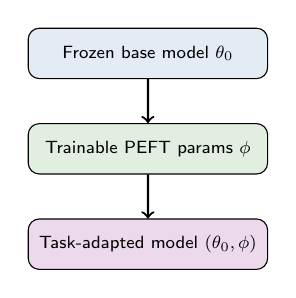
\begin{tikzpicture}[
        scale=0.8, transform shape,
        node distance=0.7cm,
        % Prefer low-saturation fills for readability in two-column papers.
        box/.style={rectangle, rounded corners, draw, fill=#1!15, text=black,
            minimum width=3.8cm,
            minimum height=0.8cm,
            align=center, font=\sffamily\footnotesize}
    ]
        \node[box=qubitblue] (node1) {Frozen base model $\theta_0$};
        \node[box=aigreen, below=of node1] (node2) {Trainable PEFT params $\phi$};
        \node[box=quantumpurple, below=of node2] (node3) {Task-adapted model $(\theta_0,\phi)$};
        
        % Connections
        \draw[->, thick] (node1) -- (node2);
        \draw[->, thick] (node2) -- (node3);
    \end{tikzpicture}
    \caption{A unifying view of PEFT: keep base parameters frozen and learn a small adaptation parameter set.}
    \label{fig:peft-schematic}
\end{figure}

%%%%%%%%%%%%%%%%%%%%%%%%%%%%%%%%%%%%%%%%%
% DESIGN SPACE + COMPOSITION
%%%%%%%%%%%%%%%%%%%%%%%%%%%%%%%%%%%%%%%%%
\section{Design Space and Method Composition (2022--2026)}
The effectiveness of PEFT depends not only on the family of parameterization but also on design decisions such as \emph{where} to apply updates, \emph{how} to allocate a parameter budget, and \emph{how} to compose multiple specialized modules \cite{chen2023parameter,han2024parameter}. This section summarizes the most common axes that recur across 2022--2026 work.

\subsection{Where to Adapt: Placement and Target Matrices}
Design-space studies emphasize that updating different parts of a transformer can lead to markedly different trade-offs, and that the best placement can depend on modality and task \cite{chen2023parameter,xin2024parameter}. In LLMs, LoRA-style updates are often inserted into attention projections and/or feed-forward layers, while adapter-style modules may be placed after sublayers; in vision and multimodal models, prompt tokens and lightweight adapter blocks are frequently compared as competing adaptation interfaces \cite{hu2021lora,houlsby2019parameter,jia2022visual,chen2022adaptformer}.

\subsection{Budget Allocation: Rank and Layer Selection}
Given a fixed parameter budget, rank allocation across layers can be optimized rather than set uniformly. Adaptive schemes allocate higher rank to more ``important'' layers or training dynamics, improving performance under the same budget \cite{zhang2023adalora,liu2024dora}. Related analyses argue that understanding which directions matter for task adaptation can inform initialization and budget placement, connecting PEFT design to representation geometry \cite{si2024task,afzal2026linearization}.

\subsection{Initialization, Optimization, and Stability}
Recent work suggests that optimization details---initialization, scaling factors, and training dynamics---can dominate naive comparisons between PEFT families \cite{wang2024lora,meng2024periodiclora}. Theoretical and empirical analyses also illuminate limitations of low-rank constraints and help explain when PEFT behaves similarly to (or diverges from) full fine-tuning \cite{hu2024computational,afzal2026linearization}.

\subsection{Composition, Continual Adaptation, and Interference}
When multiple adapters or low-rank modules are trained for different tasks, composition strategies must mitigate interference. Non-destructive composition (e.g., adapter fusion) and merging-based approaches (e.g., TIES-style merging) provide complementary options, but both introduce new evaluation requirements and failure modes \cite{pfeiffer2020adapterfusion,yadav2023ties,gauthiercaron2024merging}. Continual PEFT and multi-task settings further amplify these challenges, motivating surveys and benchmarks for continual adaptation \cite{coleman2025parameter}.

%%%%%%%%%%%%%%%%%%%%%%%%%%%%%%%%%%%%%%%%%
% SYSTEMS VIEW
%%%%%%%%%%%%%%%%%%%%%%%%%%%%%%%%%%%%%%%%%
\section{Systems View: Training and Serving Efficiency}
PEFT algorithms are often adopted because they change the \emph{systems} constraints of post-training. Training-time memory is frequently dominated by optimizer states for trainable parameters; reducing the number of trainable parameters can therefore enable much larger backbones under the same hardware budget, even when activations still dominate at long context lengths \cite{dettmers2023qlora,han2024parameter}. Serving-time efficiency depends on whether the adaptation introduces extra compute (adapter blocks, side modules) and whether the learned updates can be merged into base weights (as is common for LoRA-style linear deltas) \cite{hu2021lora,houlsby2019parameter}.

In practice, the benefits are largest when optimizer states dominate; for very long sequences or large batch sizes, activation memory and attention KV-cache can still be the bottleneck. This motivates reporting not only trainable-parameter counts but also peak activation/KV memory under the target context length, and clarifying whether techniques such as gradient checkpointing are used \cite{han2024parameter,prottasha2025peft}. A second systems axis is \emph{mergeability}: LoRA-style linear deltas can often be materialized into the base weights for inference, whereas adapter blocks introduce extra compute and may require runtime routing and caching to keep latency low \cite{hu2021lora,houlsby2019parameter,pfeiffer2020adapterhub}.

\begin{figure}[t]
    \centering
    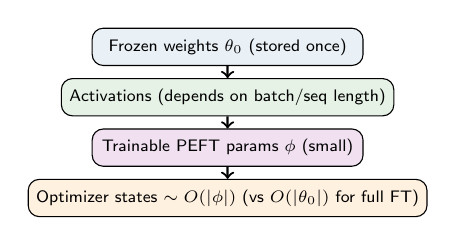
\begin{tikzpicture}[
        scale=0.86, transform shape,
        node distance=0.18cm,
        box/.style={rectangle, rounded corners, draw, fill=#1!12, text=black,
            minimum width=4.0cm,
            minimum height=0.55cm,
            align=center, font=\sffamily\scriptsize}
    ]
        \node[box=qubitblue] (w) {Frozen weights $\theta_0$ (stored once)};
        \node[box=aigreen, below=of w] (a) {Activations (depends on batch/seq length)};
        \node[box=quantumpurple, below=of a] (p) {Trainable PEFT params $\phi$ (small)};
        \node[box=errororange, below=of p] (o) {Optimizer states $\sim O(|\phi|)$ (vs $O(|\theta_0|)$ for full FT)};
        \draw[->, thick] (w) -- (a);
        \draw[->, thick] (a) -- (p);
        \draw[->, thick] (p) -- (o);
    \end{tikzpicture}
    \caption{A practical memory view: PEFT primarily reduces optimizer-state memory by restricting trainable parameters \cite{dettmers2023qlora,han2024parameter}.}
    \label{fig:peft-memory}
\end{figure}

\subsection{Quantized Fine-Tuning and QLoRA-Style Pipelines}
Quantized PEFT combines low-bit quantization of the frozen backbone with a small trainable adapter (often LoRA) to reduce memory while retaining gradient-based adaptation \cite{dettmers2023qlora}. This shifts practical feasibility: models that previously required multi-GPU full fine-tuning can be adapted on a single high-memory GPU, at the cost of additional implementation and reproducibility details (quantization scheme, compute dtype, and optimizer choices) \cite{han2024parameter,prottasha2025peft}.

In systems practice, small configuration differences can dominate outcomes: quantization format and kernels, activation checkpointing, gradient accumulation, and optimizer implementations all affect peak memory and throughput. Since LoRA rank and placement translate into extra matrix multiplications unless updates are merged, throughput reporting should clarify whether adapters are kept separate at inference or materialized into the backbone weights \cite{hu2021lora,dettmers2023qlora,prottasha2025peft}.

\begin{figure}[t]
     \centering
     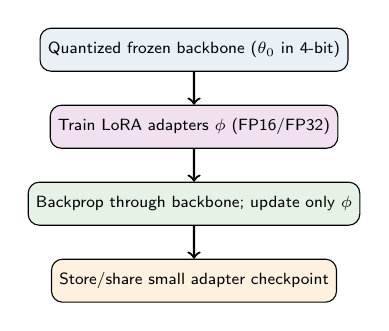
\begin{tikzpicture}[
        scale=0.84, transform shape,
        node distance=0.5cm,
        box/.style={rectangle, rounded corners, draw, fill=#1!12, text=black,
            minimum width=4.0cm,
            minimum height=0.65cm,
            align=center, font=\sffamily\scriptsize}
    ]
        \node[box=qubitblue] (base) {Quantized frozen backbone ($\theta_0$ in 4-bit)};
        \node[box=quantumpurple, below=of base] (lora) {Train LoRA adapters $\phi$ (FP16/FP32)};
        \node[box=aigreen, below=of lora] (train) {Backprop through backbone; update only $\phi$};
        \node[box=errororange, below=of train] (ckpt) {Store/share small adapter checkpoint};
        \draw[->, thick] (base) -- (lora);
        \draw[->, thick] (lora) -- (train);
        \draw[->, thick] (train) -- (ckpt);
    \end{tikzpicture}
    \caption{A simplified QLoRA-style pipeline: quantize the frozen backbone and optimize only adapter parameters \cite{dettmers2023qlora}.}
    \label{fig:qlora-pipeline}
\end{figure}

\subsection{Serving, Hot-Swapping, and Multi-Adapter Routing}
In production, PEFT enables maintaining a shared backbone and swapping small modules per user or domain, but it introduces management problems such as versioning, routing, and merge conflicts when combining multiple capabilities \cite{pfeiffer2020adapterhub,yadav2023ties}. Model and adapter merging methods provide algorithmic tools for reducing the number of deployed modules, but they require careful validation to avoid destructive interference \cite{he2023mera,gauthiercaron2024merging,yadav2024what}.

Operationally, routing introduces its own design space: systems may cache popular adapters, batch requests by adapter to reduce hot-swapping overhead, or perform periodic consolidation via merging to control the number of deployed artifacts \cite{pfeiffer2020adapterhub,yadav2023ties,gauthiercaron2024merging}. These choices tie directly to governance, since a larger adapter ecosystem increases the surface area for supply-chain attacks and makes provenance metadata and regression testing more important \cite{sun2024peftguard,liu2024loratk}.

%%%%%%%%%%%%%%%%%%%%%%%%%%%%%%%%%%%%%%%%%
% EVALUATION
%%%%%%%%%%%%%%%%%%%%%%%%%%%%%%%%%%%%%%%%%
\section{Evaluation and Benchmarks}
PEFT evaluation should jointly measure \emph{quality} and \emph{cost}. For language, standard benchmark suites (e.g., GLUE/SuperGLUE) and broad knowledge/ability tests (e.g., MMLU and BIG-bench) provide complementary signals, while dialogue-style evaluation protocols (e.g., MT-Bench-style) aim to reflect instruction-following behavior \cite{wang2018glue,wang2019superglue,hendrycks2020measuring,srivastava2022beyond,zheng2023judging}. For vision and vision-language, image classification, detection, and VQA-style tasks are common, often using ImageNet/COCO/VQA and CLIP-style retrieval settings \cite{russakovsky2014imagenet,lin2014microsoft,agrawal2015vqa,radford2021learning}.

Beyond task scores, we recommend reporting: trainable parameters, peak memory, wall-clock time, and any serving-time overhead (extra modules, extra tokens, or inability to merge) \cite{han2024parameter,chen2023parameter}. For fairness and reproducibility, PEFT comparisons should explicitly document adapter placement, rank/budget choices, optimizer and quantization settings, and data regime \cite{dettmers2023qlora,zhang2023adalora,wang2024lora}.

\begin{table}[t]
    \centering
    \caption{Recommended reporting checklist for PEFT experiments.}
    \label{tab:peft-reporting}
    \scriptsize
    \setlength{\tabcolsep}{3pt}
    \begin{tabular}{p{1.7cm}p{5.5cm}}
        \toprule
        \textbf{Category} & \textbf{Items to report} \\
        \midrule
        Base model & name/version, parameter count, context length, tokenizer \\
        Data & dataset(s), size, preprocessing, licensing, train/val split \\
        PEFT config & family, placement, rank/budget, initialization, scaling \\
        Training & optimizer, LR schedule, batch size, precision/quantization, steps \\
        Cost & peak memory, wall-clock, tokens/sec, number of GPUs \\
        Evaluation & benchmarks, prompts/templates, decoding, seeds, variance \\
        Serving & mergeability, latency overhead, module size, routing strategy \\
        \bottomrule
    \end{tabular}
\end{table}

\subsection{Benchmarks and Metrics}
Benchmark choice interacts with PEFT design: prompt-based methods may behave differently under low-data regimes and on tasks that are sensitive to input formatting, while low-rank methods are frequently tuned for instruction-following or domain adaptation at scale \cite{li2021prefix,liu2021p,hu2021lora}. We therefore recommend covering (i) classic NLU/NLG suites, (ii) broad capability tests, and (iii) instruction/dialogue protocols, alongside modality-specific evaluations for vision and multimodal models \cite{wang2018glue,hendrycks2020measuring,zheng2023judging,xin2024parameter}.

\subsubsection{Dataset and Task Coverage}
For LLMs, coverage typically spans classic NLU (e.g., GLUE-style) and broad knowledge/capability tests (e.g., MMLU/BIG-bench), but many PEFT papers also emphasize instruction tuning and domain-specific adaptation where public benchmarks may be imperfect proxies \cite{wang2018glue,hendrycks2020measuring,srivastava2022beyond,han2024parameter}. For multimodal models, evaluation often mixes general vision tasks with vision-language alignment tasks, which can make cross-paper comparisons sensitive to data, prompting templates, and protocol choices \cite{radford2021learning,prottasha2025peft}.

\subsubsection{Metric Limitations}
Scalar task scores do not capture cost and deployment constraints, and preference-based evaluations (including LLM-as-judge protocols) introduce additional sources of variance \cite{zheng2023judging}. Whenever possible, we advocate reporting cost--quality Pareto curves (or at least multiple operating points) and providing enough hyperparameter detail to allow reproduction \cite{han2024parameter,chen2023parameter}.

\subsection{Failure Modes and Robustness}
PEFT can change failure modes because small updates can have outsized behavioral effects, especially under distribution shift or repeated adaptation. Emerging work highlights safety and fairness risks of low-cost adaptation as well as security concerns such as extraction attacks against deployed adapters \cite{taraghi2025efficiency,wang2025stolenlora}. These risks motivate provenance and access-control mechanisms for adapter sharing and deployment \cite{pfeiffer2020adapterhub,taraghi2025efficiency}.

% Example table
\begin{table}[t]
\centering
\caption{Qualitative trade-offs of major PEFT families (typical patterns; details vary by implementation).}
\label{tab:peft-tradeoffs}
\scriptsize
\setlength{\tabcolsep}{3pt}
\begin{tabular}{p{1.75cm}p{1.15cm}p{1.45cm}p{1.05cm}}
\toprule
\textbf{Family} & \textbf{Train} & \textbf{Serve} & \textbf{Merge} \\
\midrule
Adapters/side & Low & Low--Med & Usually no \\
Low-rank (LoRA) & Low & Low & Often yes \\
Prompt/prefix & Very low & Med (extra tokens) & N/A \\
Selective (BitFit/IA$^3$) & Very low & None--Low & N/A \\
\bottomrule
\end{tabular}
\end{table}

%%%%%%%%%%%%%%%%%%%%%%%%%%%%%%%%%%%%%%%%%
% APPLICATIONS
%%%%%%%%%%%%%%%%%%%%%%%%%%%%%%%%%%%%%%%%%
\section{Applications and Case Studies}
PEFT has become a common ``inner loop'' for adapting open and closed foundation models. In language, LoRA and QLoRA-style recipes are widely used for instruction tuning and domain specialization under limited hardware, and adapter ecosystems support multi-task specialization with reusable modules \cite{hu2021lora,dettmers2023qlora,pfeiffer2020adapterhub}. In vision and vision-language, prompt tuning and lightweight adapters provide strong few-shot and transfer baselines for frozen backbones, especially when combined with CLIP-style pretraining \cite{jia2022visual,zhang2021tip,radford2021learning,chen2022adaptformer}.

Generative vision models provide another case study: diffusion models and diffusion transformers are frequently personalized with low-rank deltas because they offer a simple interface for user-specific concepts while keeping the base model intact \cite{ho2020denoising,rombach2021high,huang2024in}. These application patterns also highlight the need for robust evaluation and provenance, since adapter sharing and user-specific modules can leak information or be misused \cite{wang2025stolenlora,taraghi2025efficiency}.

\begin{table}[t]
    \centering
    \caption{Common PEFT patterns across modalities (representative examples).}
    \label{tab:peft-modalities}
    \scriptsize
    \setlength{\tabcolsep}{3pt}
    \begin{tabular}{p{0.85cm}p{2.2cm}p{2.4cm}}
        \toprule
        \textbf{Mod.} & \textbf{Typical interface} & \textbf{Representative refs.} \\
        \midrule
        LLM & LoRA / QLoRA; prefix & \cite{hu2021lora,dettmers2023qlora,li2021prefix} \\
        ViT & Visual prompts; adapters & \cite{jia2022visual,chen2022adaptformer} \\
        VLM & CLIP adapters; rank search & \cite{zhang2021tip,radford2021learning,chittyvenkata2025langvision} \\
        Diff. & Low-rank deltas; personalization & \cite{ho2020denoising,rombach2021high,huang2024in} \\
        \bottomrule
    \end{tabular}
\end{table}

\subsection{Instruction Tuning in LLMs and VLMs}
A representative modern recipe is: start from a pretrained backbone, optionally quantize it, and perform supervised instruction tuning by training only a small set of low-rank deltas. QLoRA-style pipelines make this feasible on limited hardware while preserving most of the quality of full fine-tuning, which accelerates iteration over data mixtures and hyperparameters \cite{dettmers2023qlora,hu2021lora}. In multimodal instruction tuning, similar low-rank interfaces are increasingly used to adapt language/cross-attention components while keeping the vision encoder frozen; design-space studies and NAS-style rank search highlight that optimal rank and placement can differ substantially across modalities \cite{jia2022visual,chen2022adaptformer,chittyvenkata2025langvision}.

At deployment time, practitioners either (i) merge deltas into base weights for a single capability, or (ii) maintain a pool of adapters and route requests by user/domain. Merging methods offer a compromise by combining many specialized deltas into fewer deployable modules, but they require regression testing because composition can introduce interference or safety regressions \cite{yadav2023ties,gauthiercaron2024merging,sun2024peftguard}.

\subsection{Diffusion Personalization and Concept Composition}
Personalizing text-to-image generation often uses per-subject fine-tuning (e.g., DreamBooth) or embedding-based methods (textual inversion); PEFT provides a lightweight alternative by storing only a low-rank delta per concept \cite{ruiz2022dreambooth,gal2022an,rombach2021high}. Recent work extends low-rank adaptation to diffusion transformers and explores in-context control of LoRA modules, enabling concept injection without modifying the base checkpoint \cite{huang2024in}. Because diffusion adapters are easily shared and composed, they inherit the same supply-chain and backdoor risks as language adapters, and the risk is arguably amplified by the difficulty of exhaustively testing image-generation behavior \cite{lyu2026when,yin2024lobam}.

\begin{table}[t]
    \centering
    \caption{Text-to-image personalization interfaces and what is shared.}
    \label{tab:diffusion-personalization}
    \scriptsize
    \setlength{\tabcolsep}{3pt}
    \begin{tabular}{p{1.55cm}p{1.35cm}p{1.65cm}p{1.55cm}}
        \toprule
        \textbf{Method} & \textbf{Trainable} & \textbf{Shared artifact} & \textbf{Typical trade-off} \\
        \midrule
        DreamBooth \cite{ruiz2022dreambooth} & many params & full checkpoint & high fidelity; heavy sharing \\
        Textual inv. \cite{gal2022an} & embeddings & small vectors & portable; limited capacity \\
        Diffusion LoRA \cite{huang2024in} & low-rank & small adapters & composable; needs audits \\
        \bottomrule
    \end{tabular}
\end{table}

%%%%%%%%%%%%%%%%%%%%%%%%%%%%%%%%%%%%%%%%%
% SAFETY / PROVENANCE
%%%%%%%%%%%%%%%%%%%%%%%%%%%%%%%%%%%%%%%%%
\section{Safety, Governance, and Provenance}
Low-cost adaptation changes the risk landscape: it becomes easier to create many specialized variants, and repeated fine-tuning can cause undesirable behavioral drift \cite{taraghi2025efficiency,han2024parameter}. In the PEFT setting, risk is amplified by \emph{artifact modularity}: adapters and low-rank deltas are easy to publish, reuse, and compose, which creates new attack surfaces and governance challenges \cite{pfeiffer2020adapterhub,liu2024loratk}.

\subsection{Threat Model: Sharing and Composing PEFT Artifacts}
PEFT encourages sharing small ``patches'' (adapters, LoRA deltas, prompt vectors) rather than entire models. This enables rapid specialization but also supports supply-chain risks where seemingly benign adapters embed malicious behaviors \cite{liu2024loratk}. Composition mechanisms (fusion, merging, routing) further complicate auditing because downstream behavior depends on how multiple modules interact \cite{pfeiffer2020adapterfusion,yadav2023ties,yin2024lobam}.

\subsection{Backdoors and Trojaned Adapters}
Recent work demonstrates that LoRA adapters can be backdoored in ways that generalize across base models or persist through reuse in share-and-play ecosystems \cite{liu2024loratk,chen2025causal}. Backdoors are also studied in compositional settings, including model merging pipelines and multimodal or text-to-image adaptation, where adversarial adapters can masquerade as harmless updates \cite{yin2024lobam,lyu2026when}. These findings suggest that PEFT should not be treated as ``safe by default'' simply because updates are low-dimensional \cite{taraghi2025efficiency,liu2024loratk}.

\subsection{Detection and Mitigation}
Defenses include both detection (e.g., adapter-level backdoor detectors) and training-time mitigation that regularizes adaptation to reduce backdoor persistence \cite{sun2024peftguard,merenciano2026weight,luong2026why}. Since PEFT artifacts are smaller than full models, it is often practical to run additional audits per adapter version (including regression tests on safety and bias) before deployment \cite{sun2024peftguard,taraghi2025efficiency}.

\subsection{Privacy and Governance}
Privacy risks arise when adaptation data is sensitive and when adapter parameters can be extracted or reverse-engineered from deployed systems \cite{wang2025stolenlora}. Differentially private fine-tuning is one mitigation direction, but it must be reconciled with PEFT design choices and deployment constraints \cite{yu2021differentially,han2024parameter}. Governance therefore includes (i) access control and provenance metadata for adapter artifacts, (ii) evaluation checklists that track safety/fairness alongside quality and cost, and (iii) policies for sharing and composing third-party adapters \cite{pfeiffer2020adapterhub,taraghi2025efficiency}.

\subsection{Provenance Metadata and Secure Distribution}
Governance requires not only access control but also high-quality provenance metadata. Inspired by model cards and datasheets, each PEFT artifact should ship with a lightweight ``adapter card'' capturing the base model, PEFT configuration, data sources, intended use, and evaluation/safety checks \cite{mitchell2018model,gebru2018datasheets}. Because PEFT encourages distributing many small files, checksums and signing can help mitigate supply-chain risks and enable reproducible merges in share-and-play ecosystems \cite{pfeiffer2020adapterhub,liu2024loratk}.

\begin{table}[t]
    \centering
    \caption{Provenance checklist for sharing PEFT artifacts (``adapter cards'').}
    \label{tab:peft-provenance}
    \scriptsize
    \setlength{\tabcolsep}{3pt}
    \begin{tabular}{p{1.55cm}p{5.65cm}}
        \toprule
        \textbf{Category} & \textbf{Recommended fields} \\
        \midrule
        Base model & name/version, license, quantization, checksum/hash \\
        PEFT artifact & method, placement, rank/budget, scaling, mergeability \\
        Training data & source, license, size, filtering, sensitive-data notes \\
        Evaluation & benchmarks, prompts/templates, seeds/variance, cost metrics \\
        Safety & red-team tests, bias checks, backdoor scan, regression suite \\
        Distribution & release channel, signature, dependency/tool versions \\
        \bottomrule
    \end{tabular}
\end{table}

Table~\ref{tab:peft-threats} summarizes common threats and corresponding checks. Notably, because PEFT updates are cheap to generate and easy to distribute, ecosystem-level governance (upload requirements, scanning, and versioning) becomes as important as any single defense method \cite{taraghi2025efficiency,liu2024loratk}.

\begin{table}[t]
    \centering
    \caption{Safety checklist for PEFT artifacts: threats and mitigations.}
    \label{tab:peft-threats}
    \scriptsize
    \setlength{\tabcolsep}{3pt}
    \begin{tabular}{p{1.35cm}p{2.40cm}p{3.45cm}}
        \toprule
        \textbf{Threat} & \textbf{Surface} & \textbf{Mitigation / checks} \\
        \midrule
        Backdoors & shared deltas; reuse & provenance/signing; regression tests; detectors \cite{liu2024loratk,sun2024peftguard} \\
        Merge attacks & merging pipelines & merging-aware audits; hold-out safety tests \cite{yin2024lobam} \\
        Extraction & deployed endpoints & access control; monitoring; extraction audits \cite{wang2025stolenlora} \\
        Privacy leakage & training data & DP or privacy filters; policy constraints \cite{yu2021differentially} \\
        \bottomrule
    \end{tabular}
\end{table}

%%%%%%%%%%%%%%%%%%%%%%%%%%%%%%%%%%%%%%%%%
% OPEN CHALLENGES + CONCLUSION
%%%%%%%%%%%%%%%%%%%%%%%%%%%%%%%%%%%%%%%%%
\section{Open Challenges and Conclusion}
\subsection{Open Challenges}
Despite rapid progress, several challenges remain open. (1) \emph{Standardized, cost-aware evaluation}: PEFT papers still vary widely in what resources and hyperparameters are reported, and consistent cost--quality reporting is needed across modalities \cite{han2024parameter,prottasha2025peft}. (2) \emph{Composition at scale}: routing, merging, and continual adaptation require principled methods to avoid interference and to enable safe reuse of specialized modules \cite{yadav2023ties,gauthiercaron2024merging,coleman2025parameter}. (3) \emph{Theory and predictability}: understanding which directions matter for adaptation, and when low-rank or selective constraints suffice, remains an active topic \cite{si2024task,afzal2026linearization,hu2024computational}. (4) \emph{Safety, privacy, and provenance}: PEFT lowers the barrier to creating variants, which raises the stakes for robust alignment, access control, and provenance of adapter artifacts \cite{taraghi2025efficiency,wang2025stolenlora}.

\subsection{Conclusion}
PEFT has matured into a cross-modality adaptation toolkit that spans modular adapters, low-rank deltas, prompt-based parameters, and selective tuning. For 2022--early 2026, the central algorithmic themes are (i) choosing an update parameterization that matches deployment constraints (mergeability and overhead), (ii) allocating limited budgets across layers and directions, and (iii) composing many specialized modules without destructive interference \cite{hu2021lora,zhang2023adalora,yadav2023ties,han2024parameter}. Continued progress will likely depend on better cost-aware benchmarks, stronger theory for adaptation dynamics, and safety/provenance infrastructure for widespread adapter sharing \cite{prottasha2025peft,si2024task,taraghi2025efficiency}.

%%%%%%%%%%%%%%%%%%%%%%%%%%%%%%%%%%%%%%%%%
% BIBLIOGRAPHY
%%%%%%%%%%%%%%%%%%%%%%%%%%%%%%%%%%%%%%%%%
% Keep this label for page-count reporting in scripts/compile_paper.py.
\label{ReferencesStart}
\bibliographystyle{ieeetr}  
\bibliography{ref} % References are in ref.bib

\end{document} 
